% This is Latex code for the Connour et al 2020 paper.

%%%%%%%%%%%%%%%%%%%%%%%%%%%%%%%%%%%%%%%%%%%%%%%%%%%%%%%%%%%%%%%%%%%%%%%%%%%%
% AGUJournalTemplate.tex: this template file is for articles formatted with LaTeX
%
% This file includes commands and instructions
% given in the order necessary to produce a final output that will
% satisfy AGU requirements, including customized APA reference formatting.
%
% You may copy this file and give it your
% article name, and enter your text.
%
%
% Step 1: Set the \documentclass
%
%

%% To submit your paper:
\documentclass[draft]{agujournal2019}
\usepackage{url} %this package should fix any errors with URLs in refs.
\usepackage{lineno}
\usepackage[finalnew]{trackchanges} %use "inline" or "finalnew"
\usepackage{soul}
\usepackage{xcolor}
\linenumbers
% Use these is trackchanges is "inline"
%\soulregister\ref7
%\soulregister\cite7

% Future note: \remove{} add a space so remove spaces after \remove{}

%%%%%%%
% As of 2018 we recommend use of the TrackChanges package to mark revisions.
% The trackchanges package adds five new LaTeX commands:
%
%  \note[editor]{The note}
%  \annote[editor]{Text to annotate}{The note}
%  \add[editor]{Text to add}
%  \remove[editor]{Text to remove}
%  \change[editor]{Text to remove}{Text to add}
%
% complete documentation is here: http://trackchanges.sourceforge.net/
%%%%%%%

\draftfalse

\journalname{Geophysical Research Letters}

\begin{document}

\title{Mars' Twilight Cloud Band: A New Cloud Feature Seen during the Mars Year 34 Global Dust Storm}

 \authors{
 Kyle Connour\affil{1}, 
 Nicholas M. Schneider\affil{1}, 
 Zachariah Milby\affil{1}, 
 Fran\c{c}ois Forget\affil{2}, 
 Mohamed Alhosani\affil{2}, 
 Aymeric Spiga\affil{3}, 
 Ehouarn Millour\affil{2}, 
 Franck Lef{\`e}vre\affil{4},
 Justin Deighan\affil{1}, 
 Sonal K. Jain\affil{1}, 
 Michael J. Wolff\affil{5}
 }
%\thanks{*put a thanks here}   this goes after Kyle Connour\affil{1} if I choose to include it

\affiliation{1}{Laboratory for Atmospheric and Space Physics, University of Colorado, Boulder, Colorado, USA.}
\affiliation{2}{\textit{Laboratoire de M{\'e}t{\'e}orologie Dynamique/IPSL, Sorbonne Universit{\'e}, {\'E}cole Normale sup{\'e}rieure}, PSL Research University, \textit{{\'E}cole Polytechnique}, Paris, France.}
\affiliation{3}{\textit{Laboratoire de M{\'e}t{\'e}orologie Dynamique/IPSL, Institut Universitaire de France, Sorbonne Universit{\'e}, {\'E}cole Normale sup{\'e}rieure}, PSL Research University, \textit{{\'E}cole Polytechnique}, Paris, France.}
\affiliation{4}{\textit{Laboratoire Atmosph{\`e}res, Milieux, Observations Spatiales (LATMOS)}, CNRS, \textit{Sorbonne Universit{\'e}}, UVSQ, Paris, France.}
\affiliation{5}{Space Science Institute, Boulder, Colorado, USA.}

\correspondingauthor{\remove{Kyle}\add{K.} Connour}{kyle.connour@colorado.edu}

\begin{keypoints}
  \item We observed a new cloud formation phenomenon just after sunset during the Mars year 34 global dust storm in MAVEN/IUVS images
  \item Global climate model simulations are able to reproduce several but not all aspects of our observations
  \item We infer these twilight clouds formed due to semidiurnal thermal tides 
\end{keypoints}

%%%%%%%%%%%%%%%%%%%%%%%%
%%% Abstract
%%%%%%%%%%%%%%%%%%%%%%%%
% The abstract can be 150 words maximum for GRL
\begin{abstract}
We report a new water-ice cloud feature observed during the Mars year 34 global dust storm: twilight cloud bands that routinely formed just past the evening terminator. We use images taken by the MAVEN/IUVS instrument. These bands were often latitudinally-continuous, spanning over 6000~km and were present between 18:00 and 19:00 local time. They were present for nearly the entire time IUVS imaged the evening terminator and often reached altitudes of at least 40 to 50~km during the mature phase of the storm. We compare these observations to LMD global climate model simulations. The simulations generally contain the temporal and spatial extents of the bands seen in IUVS data throughout the storm, but there are some discrepancies. We infer these clouds formed as a result of semidiurnal thermal tides.
\end{abstract}

%%%%%%%%%%%%%%%%%%%%%%%%
%%% Plain language summary
%%%%%%%%%%%%%%%%%%%%%%%%
% The PLS can be 200 words maximum for GRL
\section*{Plain Language Summary}
Water-ice clouds and dust are among the most common particles in the Martian atmosphere, but the effect of global dust storms on cloud formation is largely unknown. We observed cloud bands that repeatedly formed near dusk during the Mars year 34 global dust storm. We saw these bands throughout the storm at locations all across the planet. We investigate this feature by using a global climate model, which predicted the formation of these cloud bands as a result of rapidly changing temperatures. The simulations of the bands contain several features seen in our observations, but not all.

%%%%%%%%%%%%%%%%%%%%%%%%
%%% Introduction
%%%%%%%%%%%%%%%%%%%%%%%%
\section{Introduction}
Dust storms are one of the most dynamic phenomena that occur on Mars and the increased heating they cause has a significant impact on water-ice cloud formation. During the perihelion season dust is swept into the atmosphere and localized storms can grow to regional or even global dust storms (GDSs; synonymous with the terminology adopted by \citeA{MarsAtm_The_Mars_Dust_Cycle}). The atmosphere experiences significant warming during GDSs: temperatures can increase by tens of degrees around 25~km \cite{Conrath75, Smith02} and thereby raise the condensation altitudes of water-ice clouds higher than normal. Turbulent mixing of water vapor with dust, combined with the lack of a cloud-forming cold trap, allows water vapor to reach higher altitudes during GDSs thereby permitting cloud formation above the storms. Previous studies note likely detections of thin, water-ice cloud hazes above GDSs \cite{Strausberg05, Clancy10}, but none have seen repeatable cloud features despite observations of increased high-altitude water abundances during GDSs \cite{Federova18}.

Thermal tides may play an important role in the formation of water-ice clouds during GDSs. These tides are planetary-scale gravity waves caused by the atmospheric response to aerosol heating and cooling, and are strongest during GDSs \cite{MarsAtm_The_Global_Circulation}. Previous work has found that cloud formation is closely coupled to thermal tides in the absence of GDSs \cite{Wilson14, MarsAtm_The_Global_Circulation, Hartwick19} but their relationship during GDSs remains largely unexplored. 

The Mars year (MY)~34 GDS was observed by complimentary instrument suites aboard multiple spacecraft. The dust storm began in the northern hemisphere around solar longitude ($\mathrm{L_s}$) 185$^\circ$ \cite{Sanchez_this_issue} and transitioned from the growth phase to the mature phase around $\mathrm{L_s}$ 198$^\circ$. During this phase, zonal mean temperatures increased from 195~K to 220~K in less than a week at around 40~km altitude though local temperatures varied across the planet \cite{Guzewich_this_issue, Kass_this_issue}. During these phases the warmest regions of the atmosphere moved from the southern tropics to southern high latitudes. The storm entered the decay phase around $\mathrm{L_s}$ 213$^\circ$ and remained so until after $\mathrm{L_s}$ 250$^\circ$. The temperature structures and optical depths of this storm were similar to those observed during the MY~25 GDS \cite{Kass_this_issue}, suggesting repeatable phenomenology between the storms. The MY~34 GDS is of particular interest because instruments measured vertical profiles of water vapor \cite{Aoki_this_issue} and dust \cite{Klein_this_issue}, which will allow for a detailed interrogation of the dynamics of clouds and thermal tides during this GDS.

In this study we present the first observations of twilight cloud bands that routinely formed just past the evening terminator during the MY~34 GDS. All observations come from data taken by the Imaging Ultraviolet Spectrograph (IUVS) instrument aboard the Mars Atmosphere and Volatile EvolutioN (MAVEN) spacecraft. We also ran the \textit{Laboratoire de M\'et\'eorologie Dynamique} (LMD) global climate model (GCM) with the MY~34 GDS scenario to compare with our observations. We discuss comparisons between observations and simulations as well as the role of thermal tides in the creation of these clouds.

%%%%%%%%%%%%%%%%%%%%%%%%
%%% The IUVS instrument
%%%%%%%%%%%%%%%%%%%%%%%%
\section{The IUVS Instrument}
The IUVS instrument is a scanning-slit spectrograph capable of taking composite images of Mars \cite{McClintock15, Schneider18}. For this work we use disk images taken near MAVEN's orbital apoapsis in the mid-ultraviolet (MUV) spectral channel spanning from 205 to 306~nm. At MAVEN's apoapsis nadir each pixel subtended 7~km by 7~km of the Martian surface. These images were taken in six separate swaths which sometimes contain spatial gaps when projected geographically. The apoapse observing mode lasted 70 minutes, so all images created from these data should be viewed as a composite image rather than an instantaneous snapshot in time. IUVS took data during nearly every orbit with a cadence of approximately 4.5 hours, allowing it to image recurring phenomena.

Due to MAVEN's orbit slowly precessing in local time, we observed an increasingly illuminated planet during the growth and mature phases of the MY~34 GDS. MAVEN was in a nearly polar orbit before the start of the GDS. At the onset of the storm we observed a 20\%-illuminated Martian disk. Over the next month the orbit precessed such that by the time the storm reached the decay phase the disk was fully illuminated, thereby prohibiting additional measurements of the evening terminator for the remainder of the storm. This unique orbit allowed IUVS to obtain broad spatial coverage as it scanned over the evening terminator.

%%%%%%%%%%%%%%%%%%%%%%%%
%%% Twilight cloud observations
%%%%%%%%%%%%%%%%%%%%%%%%
\section{Twilight Cloud Observations}
IUVS routinely imaged illuminated bands of aerosols which formed in twilight just past the evening terminator during the MY~34 GDS. See Figure \ref{observation_geometry} for example observations of this band with a schematic interpretation of IUVS viewing geometry. These features' appearances are characterized by the presence of a dark region at solar zenith angles greater than 90$^\circ$---indicative of clear air at sunlit altitudes---adjacent to a faint band at higher solar zenith angles where aerosols must be present at higher altitudes in order to be illuminated. These bands often spanned at least 6000~km parallel to the terminator and formed between 18:00 and 19:00. We have never previously observed a discrete aerosol feature as spatially or seasonally extended as the ones presented here.

The bands exhibited temporal and spatial differences throughout the observed phases of the storm. At the onset of the growth phase, aerosols were lofted to high altitudes at low- to mid-latitudes and around this time the first band formed (with the first unambiguous detection during orbit 7152 at $\mathrm{L_s}$ 186$^\circ$), although bands did not routinely form until $\mathrm{L_s}$ 190$^\circ$. They were often distinctly present from this time until the latter half of the mature phase, when they were occasionally absent and more difficult to discern, and became more distinctive again during the decay phase for the remainder of the time IUVS imaged over the evening terminator (with the last unambiguous detection during orbit 7425 at $\mathrm{L_s}$ 217$^\circ$). The bands were often latitudinally continuous and displayed no obvious meridional brightness variations. However, they had characteristics that varied with longitude. Between 330$^\circ$ and 90$^\circ$ east longitude they were more likely to be patchy or completely absent than at all other longitudes. Between longitudes of 120$^\circ$ and 210$^\circ$ they were most likely to be present and most easily discernible. Between longitudes of 240$^\circ$ and 300$^\circ$ (near the Tharsis region), thin, streaky aerosols straddled the day/night boundary and appeared to merge with the bands, making them harder to discern.

\begin{figure}[ht!]
    \centerline{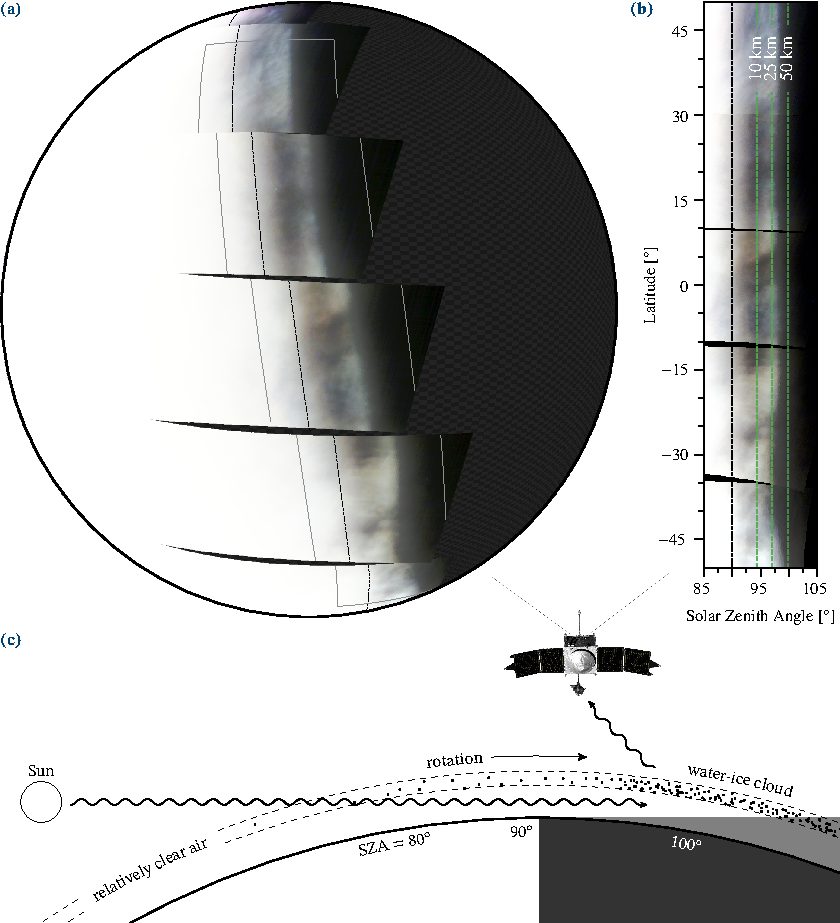
\includegraphics[width=\textwidth]{observation_geometry.pdf}}
    \caption{Composite graphic describing our observations, illuminated altitudes, and physical interpretation of a twilight cloud band. (a) Example projection of a latitudinally-continuous twilight cloud band taken shortly after the start of the mature phase of the GDS (orbit 7281; $\mathrm{L_s}$ 200$^\circ$). This false-color projection represents what each swath would have looked like when viewed from the position of the spacecraft at apoapsis. The black dashed line denotes the location of the terminator and the gray box denotes the bounds of Figure \ref{observation_geometry}b. (b) Minimum illuminated altitudes of the cloud band. We convert solar zenith angles into minimum altitudes at which these aerosols must be directly illuminated, which reveals bands often reached altitudes of at least 40 to 50~km. (c) A schematic, cross-sectional representation of IUVS viewing geometry. Incoming ultraviolet solar radiation did not interact with water vapor and encountered few, if any, water-ice clouds before illuminating this band from below. Some light was scattered through these clouds directly to the spacecraft. Schematic not to scale.}
    \label{observation_geometry}
\end{figure}

We examine altitudes as a first step in determining the composition of the bands. When present they were visible at solar zenith angles between 95$^\circ$ and 100$^\circ$. We convert solar zenith angles into minimum altitudes at which these bands could be directly illuminated from below, derived as in Figures \ref{observation_geometry}b and \ref{sza_alts_composite}. The solar zenith angles reported in IUVS data products are the surface solar zenith angles of a reference ellipsoid. We calculate the altitude of the planet's shadow at these solar zenith angles to determine the minimum altitude at which these aerosols must be to be directly illuminated. For example, observations during the growth phase of this storm show patchy bands present at altitudes of at least 10 to 25~km. As the storm reached the mature phase these aerosols regularly reached altitudes of at least 40 to 50~km. Despite zonal brightness variations, these altitudes are independent of longitude. If these clouds formed a uniform layer above the planet and crossed the planet's shadow, the greatest minimum illuminated altitude is their maximum altitude. If this assumption is reasonable, these altitudes rule out a $\mathrm{CO_2}$-ice composition because $\mathrm{CO_2}$-ice clouds normally form at altitudes higher than 50~km and the increased warming from the global dust storm makes their formation more implausible \cite{Clancy98, Clancy19}.

\begin{figure}[ht!]
    \centerline{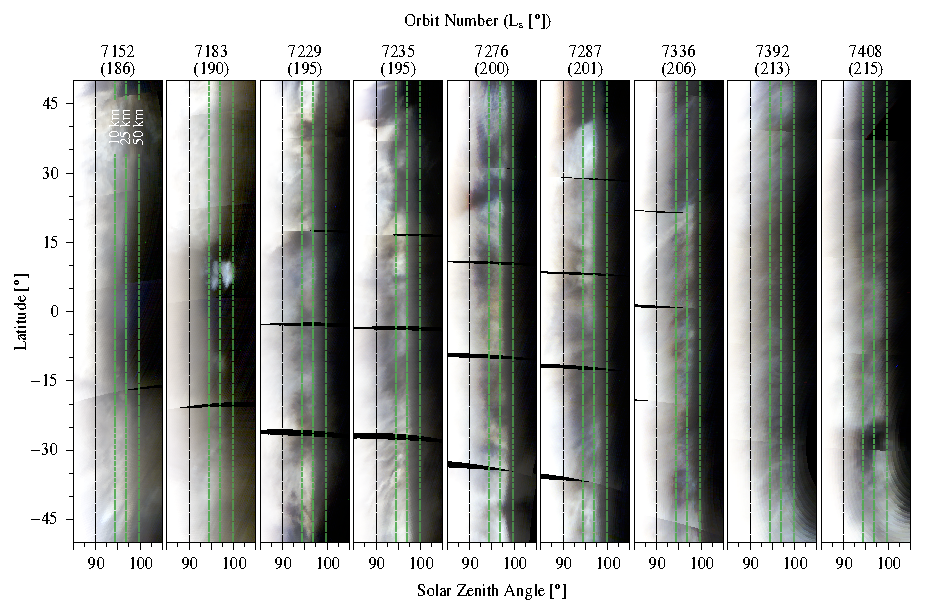
\includegraphics[width=\textwidth]{sza_alts_composite.pdf}}
    \caption{Seasonal detections of twilight cloud bands throughout the GDS. Early observations show aerosols lofted to high altitudes at mid-latitudes. Toward the end of the growth phase the bands regularly appeared and as the storm matured, these clouds were more likely to form continuous bands. Each orbit has an individualits own color stretch to bring out contrast in the range of pixels bounding the bands. Orbit 7392 shows an image with no discernible cloud band, indicating this phenomenon is not always observed. In all panels the dashed black line denotes the location of the terminator.}
    \label{sza_alts_composite}
\end{figure}

We examine the spectral signatures and morphologies of the bands to determine if they were comprised of water ice or dust. If they were comprised of dust, we would expect only brightness variations between them and dayside dust; however when they are present in IUVS data they show a disproportionate increase in signal at shorter wavelengths in MUV spectra. Compared to optically-thick dust, water-ice clouds show the most significant reflectance enhancements at the short-wavelength end of MUV spectra \cite{Willame17, Wolff19}, supporting a water-ice composition. Their morphologies also point to a water-ice composition. If the bands were composed of dust, there would have needed to be ongoing terminator upwelling that consistently raised dust to altitudes of at least 25 to 50~km while simultaneously creating streaks of dust at high altitudes crossing the dark band. We find this scenario implausible. We find it more plausible that either streaky water-ice clouds above the GDS crossed the dark regions and merged with the bands or thermal irregularities only allowed cloud formation in the observed morphologies.

%%%%%%%%%%%%%%%%%%%%%%%%
%%% Model results and discussions
%%%%%%%%%%%%%%%%%%%%%%%%
\section{Model Results and Discussion}
We interpret IUVS observations with simulations from the LMD GCM \cite{Forget99} using conditions designed to replicate the MY~34 GDS. Using the same methodology as \citeA{Montabone_this_issue} we prescribed the spatial and temporal dust optical depths using a dust climatology derived from available observations \cite{Montabone15}. \citeA{Klein_this_issue} and \citeA{Montabone_this_issue} analyze this MY~34 GDS simulation in more detail. We prescribed column optical depths but allowed the vertical dust optical depths to evolve through the semi-interactive dust transport scheme described in \citeA{Madeleine11}. Water-ice cloud radiative effects and microphysics are described in \citeA{Madeleine12} and \citeA{Navarro14}. Simulations were output every 15 minutes for each sol (Martian days since $\mathrm{L_s}$ 0$^\circ$).

These simulations show both diurnal and seasonal differences between clouds before and during the storm (Figures \ref{lmd_diurnal_profiles} and \ref{lmd_seasonal_profiles}). Here we restrict our discussion to equatorial and mid-latitudes since those were the latitudes IUVS most thoroughly imaged. Before the storm the simulated atmospheres were relatively cold, producing thin clouds during the day and thicker clouds between 20 and 30~km altitude at night. During the growth phase the storm was generally too warm to allow for repeatable cloud formation but around sol 400 ($\mathrm{L_s}$ 197$^\circ$; when the storm reached the mature phase) the dust distribution evolved to allow for colder temperatures and therefore permit repeatable cloud formation. During the early parts of the mature phase, clouds formed between altitudes of 50 and 80~km during day, then dropped tens of kilometers around dusk. This transient phenomenon lasted through some or most of the mature phase in the middle atmosphere, depending on latitude, before clouds became thin or nonexistent. At these times the changing dust distribution permitted clouds almost exclusively between longitudes of 240$^\circ$ and 90$^\circ$ between northern low- and -mid-latitudes. Similarly, they permitted clouds almost exclusively between longitudes of 120$^\circ$ and 300$^\circ$ at southern low- to mid-latitudes.

\begin{figure}[ht!]
    \centerline{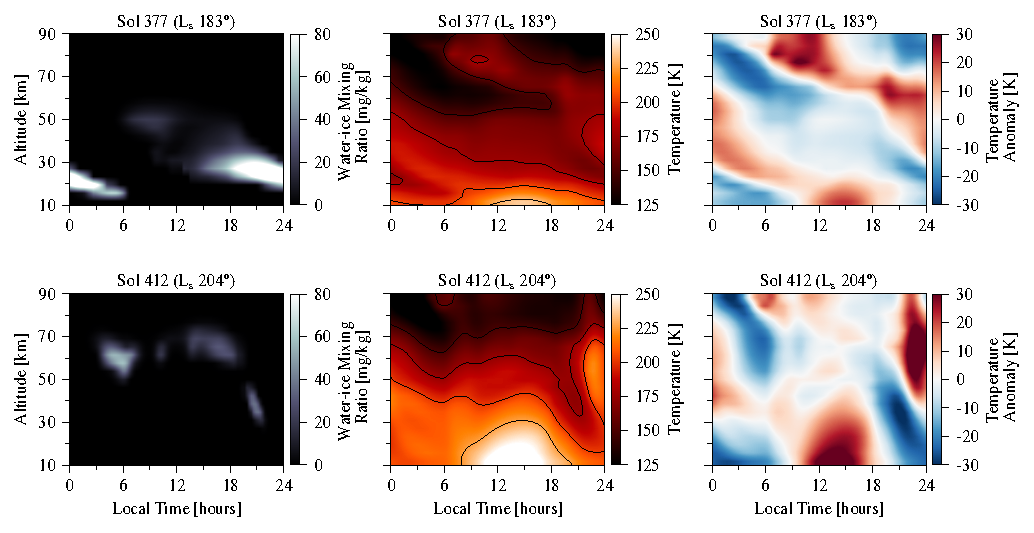
\includegraphics[width=\textwidth]{lmd_2018_dust_storm_diurnal_profiles.pdf}}
    \caption{LMD GCM simulations of the diurnal evolution of the atmosphere at the equator and 249$^\circ$~E during $\mathrm{L_s}$ 183$^\circ$ (top; before the MY~34 GDS) and $\mathrm{L_s}$ 204$^\circ$ (bottom; during the peak of the mature phase and corresponding to the terminator in Figure \ref{data_model}). These figures show cross-sections as a function of altitude above the areoid [km] at local true solar time. (left): Water-ice cloud mixing ratios [mg of ice per kg of air]. (middle): Temperature [K]. (right): Temperature anomaly (difference between the instantaneous temperature and the diurnal mean temperature at each altitude, in [K]) showing the signature of thermal tides. Clouds show seasonal variability, forming at low altitudes during the night before the storm and forming at high altitudes during the day with decreasing altitudes around dusk during the storm.}
    \label{lmd_diurnal_profiles}
\end{figure}

\begin{figure}[ht!]
    \centerline{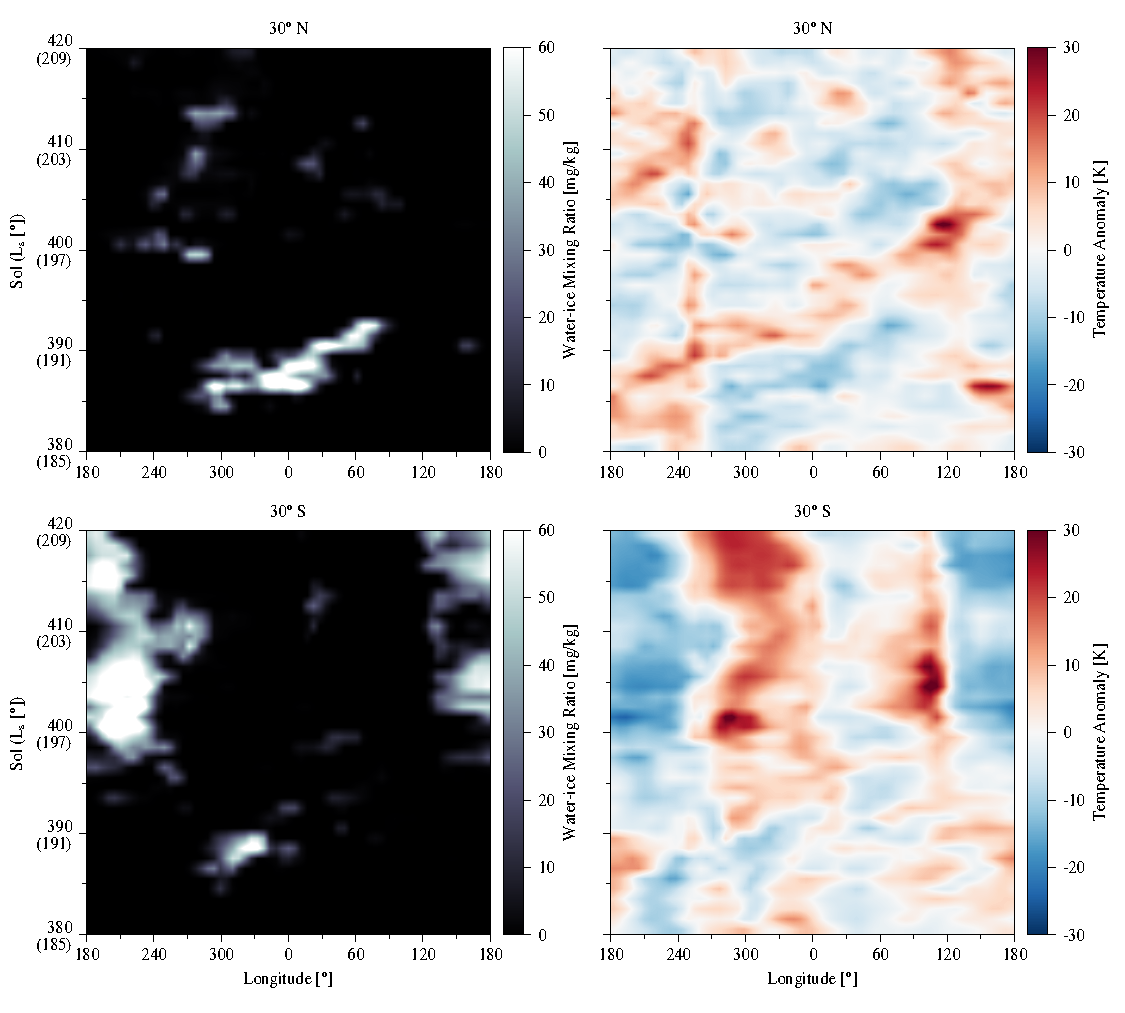
\includegraphics[width=\textwidth]{lmd_2018_dust_storm_seasonal_profiles.pdf}}
    \caption{Simulated cloud formation and corresponding temperature anomalies during the growth and mature phases of the MY~34 global dust storm at 30$^\circ$~N (top) and 30$^\circ$~S (bottom) at 19:00 local time. (left) Water-ice mass mixing ratio at 60~km above the dusk terminator. (right) Temperature anomalies at the same altitude and local time. Temperatures evolved with changing dust distributions, with colder temperatures and more clouds present after sol 400 ($\mathrm{L_s}$ 197$^\circ$). Throughout the storm, cloud formation was strongly correlated with negative temperature anomalies.}
    \label{lmd_seasonal_profiles}
\end{figure}

Despite the coarse resolution of the simulations (3.8$^\circ$ latitude by 5.6$^\circ$ longitude), they replicate several aspects of our observations. See Figure \ref{data_model} for qualitative comparison. The simulations contain twilight clouds after the start of the mature phase---when we saw the brightest and most distinctive bands. However, we also observed repeatable twilight cloud formation throughout the latter half of the growth and mature phases, which is inconsistent with the simulations. They contain zonal structure at southern low- and mid-latitudes consistent with our observations but cannot account for this structure at equatorial or northern mid-latitudes. Therefore, the simulations often contain latitudinally-continuous bands past the terminator, but they are rarely as latitudinally-extended as our observations. Finally, although it is a loose constraint, the simulations contain clouds at altitudes consistent with our observations. If our minimum illumination altitudes are the cloud altitudes, the simulated cloud altitudes are somewhat higher than our observations; however additional measurements are needed to address this issue.

\begin{figure}[ht!]
    \centerline{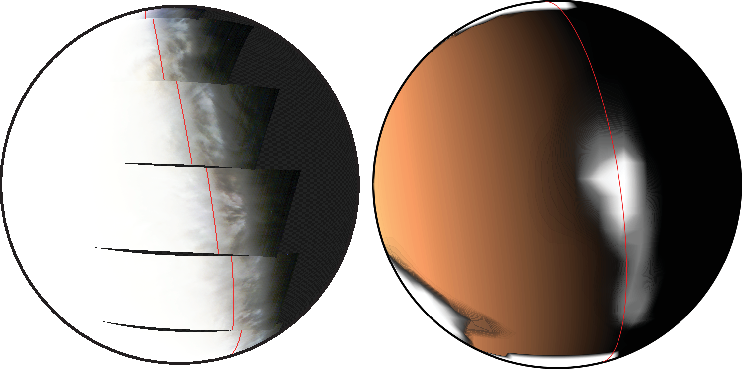
\includegraphics[width=\textwidth]{data_model_comparison.pdf}}
    \caption{A comparison between an IUVS projection (left) and an LMD GCM simulation (right). We enhanced the IUVS projection for orbit 7313 ($\mathrm{L_s}$ 204$^\circ$) at longitude of 249$^\circ$ to bring out features at high solar zenith angles, which displays both a cloud band and streaky clouds around the terminator. We created a simple relationship to view the LMD GCM simulation at the same spacecraft location and solar longitude as the IUVS image. The background layer represents the surface illumination with a brownish color proportional to the cosine of the solar zenith angle, while the foreground layer represents the ``illumination'' of the clouds through the ice mass weighted by local insolation and IUVS viewing geometry. Mathematically, this relationship is: $I_\mathrm{cloud}$ = $I_\mathrm{ice}$ $\frac{\cos \theta}{\cos \theta + \cos \phi}$ where $\theta$ is the solar zenith angle at each altitude, $\phi$ is the angle between the spacecraft-subspacecraft ray and the spacecraft-cloud ray, $I_\mathrm{ice}$ is the illuminated integrated ice column, and $I_\mathrm{cloud}$ is a proxy for the apparent mass of ice as seen by IUVS. When $\theta$ $>$ 90$^\circ$, $I_\mathrm{cloud}$ is the integration of the mass of ice at altitudes $z$ where the sun is still above the horizon, i.e., where $\theta$ $-$ $\arccos \big( \frac{R}{R+z} \big)$ $<$ 90$^\circ$, where $R$ is the radius of Mars and $z$ is the cloud altitude. The location of the terminator is shown in red in both images. The simulation contains a twilight cloud band, although it is not as latitudinally-extended as our observations.
    }
    \label{data_model}
\end{figure}

A detailed analysis of the simulations suggests the formation of these clouds was controlled by thermal tides, driven by the diurnal cycle of incoming sunlight. In a non-dusty atmosphere, the westward-propagating, diurnal tidal mode with temperature minimum in the nighttime lower atmosphere appears particularly crucial for driving the formation of the clouds. GDSs cause enhanced absorption of solar radiation, amplifying the semidiurnal tidal mode characterized by a large vertical wavelength \cite{Wilson96, Lewis05}. This triggered the formation of clouds just after twilight at higher altitudes than in clear conditions. Throughout the storm the simulations contain a wavenumber 3 tide in the longitudinal frame which allows cloud formation at discrete longitudes. This semidiurnal tidal mode created two flavors of twilight cloud bands: a ``dawn'' cloud band at most longitudes (although MAVEN's orbit precluded such apoapse observations) and a ``dusk'' cloud band at select longitudes.

%%%%%%%%%%%%%%%%%%%%%%%%
%%% Summary
%%%%%%%%%%%%%%%%%%%%%%%%
\section{Summary}
We discovered latitudinally-extensive bands of water-ice clouds just after sunset during the MY~34 GDS using IUVS data. These bands were present shortly after the start of the storm and remained present in the images through the beginning of the decay phase of the storm, although they did wane in intensity throughout the latter half of the mature phase. These clouds showed zonal brightness variability and often formed a band spanning over 6000~km. As the storm matured we found these clouds reached altitudes of at least 40 to 50~km. The spectral signatures and morphologies of the bands indicate they were comprised of water ice and not dust.

MY~34 LMD GCM simulations reproduce several of the basic features of the bands seen in IUVS images. They often display latitudinally-continuous cloud bands and southern mid-latitudes contain the bands' broad zonal variability as seen in our observations. They predict peak cloud formation rates during the beginning of the mature phase, consistent with our observations. The modeled altitudes are also in agreement with the minimum illuminated altitudes derived from the images. However, we observed clouds throughout the storm at equatorial and northern mid-latitudes, something which the simulations struggle to reproduce. We infer thermal tides drove the formation of these clouds: when the dust distribution allowed semidiurnal thermal tides, they caused enhanced cooling around twilight and thus allowed for cloud formation there. IUVS data provide further constraints on models to accurately represent thermal tides and their interactions with aerosols.

%%% End of body of article

%%%%%%%%%%%%%%%%%%%%%%%%%%%%%%%%%%%%%%%%%%%%%%%%%%%%%%%%%%%%%%%%
%
%  ACKNOWLEDGMENTS
%
% The acknowledgments must list:
%
% >>>>	A statement that indicates to the reader where the data
% 	supporting the conclusions can be obtained (for example, in the
% 	references, tables, supporting information, and other databases).
%
% 	All funding sources related to this work from all authors
%
% 	Any real or perceived financial conflicts of interests for any
%	author
%
% 	Other affiliations for any author that may be perceived as
% 	having a conflict of interest with respect to the results of this
% 	paper.
%

\acknowledgments
This work was supported by NASA through the MAVEN project. MAVEN/IUVS data files used in this work are identified as ``apoapse'', version 13, of the level 1b data available on the atmospheres node of the Planetary Data System. Simulations of the MY~34 GDS are publicly available at the Mars Climate Database project: \texttt{http://www-mars.lmd.jussieu.fr/}. All code used to create the plots in this work can be found at: \texttt{https://bitbucket.org/kconnour/twilight-cloud-band}. We thank John Wilson for his insights on waves and tides. We also thank the Research Experience for Undergraduates program at the Mohammed Bin Rashid Space Centre in Dubai.

\bibliography{tcb_bibliography}

\end{document}
